\documentclass[12pt]{extarticle}
\usepackage{import}
\import{./}{Includes}

\newcommand{\abchains}{\mathbf{Ch(Ab)}}

\begin{document}
\atitle{8}
 
\section*{Problem 1.}

\begin{center} 
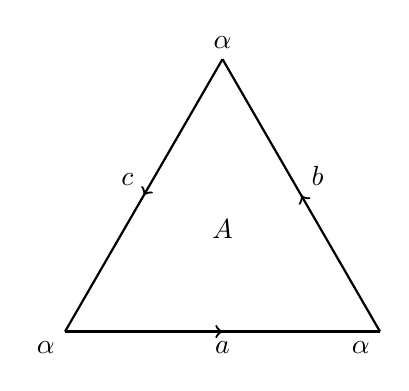
\begin{tikzpicture}
\usetikzlibrary{decorations.markings}

\begin{scope}[thick,decoration={
    markings,
    mark=at position 0.5 with {\arrow{>}}}
    ] 
    \node at (0, 1.3) {$A$};
    \draw[postaction={decorate}] (-2,0)--(2,0)
    	node[pos = 0.5, below] {$a$} node[pos = 0, below left] {$\alpha$};
    \draw[postaction={decorate}] (2,0)--(0, 3.46)
    node[pos = 0.5, above right] {$b$} node[pos = 0, below left] {$\alpha$};
    \draw[postaction={decorate}] (0,3.46)--(-2,0)
    node[pos = 0.5, above left] {$c$} node[pos = 0, above] {$\alpha$};
\end{scope}
\end{tikzpicture}
\end{center}

Let $X = \Delta^2$ with all the vertices identified at $\alpha$. Call the three ``faces'' of $\Delta^2$ which are $1$-simplices, $a$, $b$, and $c$. Finally, call the filled $2$-simplex $A$. Now consider the chain complex,
\begin{center}
\begin{tikzcd}
0 \arrow[r, "\partial_3"] & \Z A \arrow[r, "\partial_2"] & \Z a \oplus \Z b \oplus \Z c \arrow[r, "\partial_1"] & \Z \alpha \arrow[r, "\partial_0"] & 0 
\end{tikzcd}
\end{center}
The boundary maps take $\partial_2 A = a + b + c$ and $\partial_1 = 0$ because there is only one vertex so the endpoints of all $1$-simplicies are the same. Now, we can calculate the homology of this complex,
\[ H_0(\Delta) = \Z \alpha / \{0\} \cong \Z \]
\begin{align*} 
H_1(\Delta) = \ker{\partial_1}/\Im{\partial_2} =   \Z a \oplus \Z b \oplus \Z c / \left< (1, 1, 1)\right> \cong \Z \oplus \Z
\end{align*}
and finally,
\[ H_2(\Delta) = \ker{\partial_2} / \Im{\partial_3} = 0 \]

\section*{Problem 2.}

Let $X$ be the $\Delta$-complex formed by taking $\Delta^n$ and identifying all faces of the same dimension. Call $\alpha^k$ the single $k$-simplex of $X$. Therefore, the chain complex of $X$ becomes,

\begin{center}
\begin{tikzcd}
0 \arrow[r, "\partial_{n+1}"] & \Z \alpha^n \arrow[r, "\partial_{n}"] & \dots \arrow[r, "\partial_5"] & \Z \alpha^4  \arrow[r, "\partial_4"] & \Z \alpha^3 \arrow[r, "\partial_3"] & \Z \alpha^2  \arrow[r, "\partial_2"] & \Z \alpha^1 \arrow[r, "\partial_1"] & \Z \alpha^0 \arrow[r, "\partial_0"] & 0 
\end{tikzcd}
\end{center}
Since a $k$-simplex has $k + 1$ faces the boundary map acts as,
\[ \partial_k \alpha^k = \sum_{i = 0}^k (-1)^k \alpha^{k-1} = 
\begin{cases}
\alpha^{k-1} & k \text{ is even} \\
0 & k \text{ is odd}
\end{cases}\]
Therefore, 
\[ \partial_k = 
\begin{cases}
\phi_k & k \text{ is even} \\
0 & k \text{ is odd}
\end{cases}\]
where $\phi_k : \Z\alpha^k \to \Z \alpha^{k-1}$ is the map taking the generator to the generator and thus is the identity when these groups are viewed as the abstract cyclic group $\Z$. Now, consider the homology of this complex for $0 < k < n$. If $k$ is even,
\[ H_k(X) = \ker{\partial_k} / \Im{\partial_{k+1}} = \{0\}/\{0\} = 0 \]
Furthermore, if $k$ is odd,
\[ H_k(X) = \ker{\partial_k} / \Im{\partial_{k + 1}} = \Z \alpha^{k} / \Z \alpha^{k} = 0 \]
Therefore for $k < n$ we have $H_k(X) = 0$. We must now check the edge cases. For $k = 0$,
\[
H_0(X) = \Z \alpha^0 / \{0\} \cong \Z 
\]
which reflects the fact that $X$ is connected.
Finally, for $k = n$ we have,
\[ H_n(X) = \ker{\partial_n} / \Im{\partial_{n+1}} \cong \ker{\partial_n} \cong
\begin{cases}
\Z & n \text{ is odd} \\
0 & n \text{ is even}
\end{cases}\]
 

\section*{Problem 3.}

Suppose that $A$ is a retract of $X$ then there exist maps $\iota : A \hook X$ and $r : X \to A$ such that $\iota$ is the inclusion and $r \circ \iota = \id_{A}$. Since $H_n$ is a functor, $(r \circ \iota)_* = r_* \circ \iota_* = (\id_{A})_* = \id_{H_n(A)}$. Therefore, $\iota_* : H_n(A) \to H_n(X)$ is an injection and $r_* : H_n(X) \to H_n(A)$ is a surjection.  

\section*{Problem 4.}

Let $f : C \to D$ be an isomorphism in the category of $\abchains$. Therefore there is a map $g : D \to C$ such that $f \circ g = \id_{D}$ and $g \circ f = \id_C$. Therefore, $(g \circ g)_n = g_n \circ f_n = (\id_C)_n = \id_{C_n}$. Similarly, $(f \circ g)_n = f_n \circ g_n = (\id_D)_n = \id_{D_n}$. Therefore each $f_n : C_n \to D_n$ is an isomorphism of groups. 
\bigskip\\
Conversely, suppose that we have a sequence of isomorphisms of groups $f_n : C_n \to D_n$. Therefore, we have maps $g_n : C_n \to D_n$ such that $g_n \circ f_n = \id_{C_n}$ and $f_n \circ g_n = \id_{D_n}$. Therefore we have the commutative diagram, 
\begin{center}
\begin{tikzcd}
\cdots \arrow[r, "\partial_{n+3}"] & C_{n+2} \arrow[d, "f_{n+2}"] \arrow[r, "\partial_{n+2}"] & C_{n+1} \arrow[d, "f_{n+1}"]  \arrow[r, "\partial_{n+1}"] & C_{n} \arrow[d, "f_{n}"]  \arrow[r, "\partial_n"] & C_{n-1} \arrow[d, "f_{n-1}"]  \arrow[r, "\partial_{n-1}"] & C_{n-2} \arrow[d, "f_{n-2}"]  \arrow[r, "\partial_{n-2}"] & \cdots
\\
\cdots \arrow[r, "\partial_{n+3}"] & D_{n+2} \arrow[d, "g_{n+2}"] \arrow[r, "\partial_{n+2}"] & D_{n+1} \arrow[d, "g_{n+1}"]  \arrow[r, "\partial_{n+1}"] & D_{n} \arrow[d, "g_{n}"]  \arrow[r, "\partial_n"] & D_{n-1} \arrow[d, "g_{n-1}"]  \arrow[r, "\partial_{n-1}"] & D_{n-2} \arrow[d, "g_{n-2}"]  \arrow[r, "\partial_{n-2}"] & \cdots
\\
\cdots \arrow[r, "\partial_{n+3}"] & C_{n+2} \arrow[r, "\partial_{n+2}"] & C_{n+1} \arrow[r, "\partial_{n+1}"] & C_{n} \arrow[r, "\partial_n"] & C_{n-1} \arrow[r, "\partial_{n-1}"] & C_{n-2} \arrow[r, "\partial_{n-2}"] & \cdots
\end{tikzcd}
\end{center}
The squares commute because,
\begin{align*}
(g_{n} \circ f_{n}) \circ \partial_{n+1} & = g_{n} \circ (f_{n} \circ \partial_{n+1}) = g_{n} \circ (\partial_{n+1} \circ f_{n+1})
\\
& = (g_{n} \circ \partial_{n+1}) \circ f_{n+1} = \partial_{n+1} \circ (g_{n+1} \circ f_{n+1})
\end{align*}
However, $g_{n} \circ f_{n} = \id_{C_n}$ so $g \circ f = \id_C$. An identical argument shows that $f \circ g = \id_{D}$. Therefore, $f$ is an isomorphism in the category $\abchains$.

\section*{Problem 5.}
Suppose we have a complex $A$ given by,
\begin{center}
\begin{tikzcd}
\cdots \arrow[r, "\partial_7"] & A_6 \arrow[r, "\partial_6"] & A_5 \arrow[r, "\partial_5"] & A_4 \arrow[r, "\partial_4"] & A_3 \arrow[r, "\partial_3"] & A_2 \arrow[r, "\partial_2"] & A_1 \arrow[r, "\partial_1"] & A_0 \arrow[r, "\partial_0"] & 0 
\end{tikzcd}
\end{center}
such that each boundary map is zero i.e. $\partial_i = 0$. Therefore, the homology of this complex is,
\[ H_i(A) = \ker{\partial_i}/\Im{\partial_{i+1}}  = A_i / \{e\} \cong A_i \]
because the kernel of the zero map is the entire domain and the image of the zero map is trivial. 

\section*{Problem 6.}

Consider two maps $f, g : A \to B$ in the category $\abchains$. Then we can take the sum $f + g$ to be given by the component morphisms $(f + g)_n = f_n + g_n$ of abelian groups. Now, consider the action of this map on the homology groups, $ f_* : H_n(A) \to H_n(B) $ takes,
\begin{align*}
(f+g)_*(\alpha \Im{\partial_{i+1}^A}) & = (f+g)_n(\alpha) \Im{\partial_{i+1}^B} = (f_n+g_n)(\alpha) \Im{\partial_{i+1}^B} = f_n(\alpha) \Im{\partial_{i+1}^B} + g_n(\alpha)  \Im{\partial_{i+1}^B}
\\ & = f_*(\alpha \Im{\partial_{i+1}^A}) + g_*(\alpha \Im{\partial_{i+1}^A}) 
\end{align*}
Theefore $(f + g)_* = f_* + g_*$. In other notation, $H_n(f + g) = H_n(f) + H_n(g)$. 

\section*{Problem 7.}

Let $f : C \to D$ be a morphism in $\abchains$. Define the kernel and image of $f$ as the complexes $\ker{f}$ and $\Im{f}$ given by, 

\begin{center}
\begin{tikzcd}
& 0 \arrow[d] & 0 \arrow[d] & 0 \arrow[d] & 0 \arrow[d] & 0 \arrow[d] & 
\\
\cdots \arrow[r, "\partial_{n+3}"] & \ker{f_{n+2}} \arrow[d] \arrow[r, "\partial_{n+2}"] & \ker{f_{n+1}} \arrow[d]  \arrow[r, "\partial_{n+1}"] & \ker{f_{n}} \arrow[d]  \arrow[r, "\partial_n"] & \ker{f_{n-1}} \arrow[d]  \arrow[r, "\partial_{n-1}"] & \ker{f_{n-2}} \arrow[d]  \arrow[r, "\partial_{n-2}"] & \cdots
\\
\cdots \arrow[r, "\partial_{n+3}"] & C_{n+2} \arrow[d, "f_{n+2}"] \arrow[r, "\partial_{n+2}"] & C_{n+1} \arrow[d, "f_{n+1}"]  \arrow[r, "\partial_{n+1}"] & C_{n} \arrow[d, "f_{n}"]  \arrow[r, "\partial_n"] & C_{n-1} \arrow[d, "f_{n-1}"]  \arrow[r, "\partial_{n-1}"] & C_{n-2} \arrow[d, "f_{n-2}"]  \arrow[r, "\partial_{n-2}"] & \cdots
\\
\cdots \arrow[r, "\partial_{n+3}"] & \Im{f_{n+2}} \arrow[r, "\partial_{n+2}"] \arrow[d] & \Im{f_{n+1}} \arrow[r, "\partial_{n+1}"] \arrow[d] & \Im{f_{n}} \arrow[r, "\partial_n"]\arrow[d] & \Im{f_{n-1}} \arrow[r, "\partial_{n-1}"] \arrow[d] & \Im{f_{n-2}} \arrow[r, "\partial_{n-2}"] \arrow[d] & \cdots
\\
& 0 & 0 & 0 & 0 & 0 & 
\end{tikzcd}
\end{center}
where the boundary maps are restricted to the groups $\ker{f_n}$ and $\Im{f_n}$. These maps are well-defined because if $f_{n+1}(x) = 0$ then $\partial_{n+1} \circ f_{n+1}(x) = f_{n} \circ \partial_n(x) = 0$. Therefore $\partial_{n+1} \ker{f_{n+1}} \subset \ker{f_{n}}$. Furthermore, if $y \in \Im{f_{n+1}}$ then $y = f_{n+1}(x)$ we have $\partial_{n+1}(y) = \partial_{n+1} \circ f_{n+1}(x) = f_{n} \circ \partial_{n+1}(x)$ so $\partial_{n+1}(y) \in \Im{f_{n}}$ so $\partial_{n+1} \Im{f_{n+1}} \subset \Im{f_n}$. Furthermore, the property $\partial_{n} \circ \partial_{n+1} = 0$ holds for the restricted maps so each row is a complex.
\bigskip\\
From the fundamental theorem of group homomorphisms, we can form a short exact sequence in each column and an isomorphism $\phi_n : C_n / \ker{f_n} \to \Im{f_n}$. Therefore there is a morphisms of complexes $\phi : C / \ker{f} \to \Im{f}$ given by,

\begin{center}
\begin{tikzcd}[column sep = small]
\cdots \arrow[r, "\partial_{n+3}"] & C_{n+2} /\ker{f_{n+2}} \arrow[d, "\phi_{n+2}"] \arrow[r, "\partial_{n+2}"] & C_{n+1} / \ker{f_{n+1}} \arrow[d, "\phi_{n+1}"]  \arrow[r, "\partial_{n+1}"] & C_{n} / \ker{f_{n}} \arrow[d, "\phi_{n}"]  \arrow[r, "\partial_n"] & C_{n-1} / \ker{f_{n-1}} \arrow[d, "\phi_{n-1}"]  \arrow[r, "\partial_{n-1}"] & C_{n-2} / \ker{f_{n-2}} \arrow[d, "\phi_{n-2}"]  \arrow[r, "\partial_{n-2}"] & \cdots
\\
\cdots \arrow[r, "\partial_{n+3}"] & \Im{f_{n+2}} \arrow[r, "\partial_{n+2}"] & \Im{f_{n+1}} \arrow[r, "\partial_{n+1}"] & \Im{f_{n}} \arrow[r, "\partial_n"] & \Im{f_{n-1}} \arrow[r, "\partial_{n-1}"] & \Im{f_{n-2}} \arrow[r, "\partial_{n-2}"] & \cdots
\end{tikzcd}
\end{center}
where the boundary map decends to the quotient because $\partial_{n+1} \ker{f_{n+1}} \subset \ker{f_{n}}$. Because,
\begin{align*}
\partial_{n+1} \circ \phi_{n+1}(x \ker{f_{n+1}}) & = \partial_{n+1}( f_{n+1}(x) \ker{f_{n+1}}) = \partial_{n+1}(f_{n+1}(x)) \ker{f_{n}} 
\\
& = f_{n}(\partial_{n+1}(x)) \ker{f_{n}} = f_n \circ \partial_{n+1}(x \ker{f_{n+1}}) 
\end{align*}
the squares commute so $\phi$ is a morphism in $\abchains$. However, each $\phi_n$ is an isomorphism so by problem 4, $\phi : C / \ker{f} \to \Im{f}$ is an isomorphism of complexes. 


\end{document}
